\begin{framed}

Objetivos:
\begin{itemize}
    \item Describir el mecanismo de separación de capa límite.
    \item Predecir la separación de la capa límite.
    \item Calcular la fuerza sobre cuerpos sumergidos no aerodinámicos.
\end{itemize}

Contenidos:
\begin{itemize}
    \item El mecanismo de separación de capa límite.
    \item El factor de forma y su influencia en la separación de la capa límite.
    \item El arrastre por fricción y el arrastre por presión.
    \item Coeficiente de arrastre.
\end{itemize}

Bibliografía:
\begin{itemize}
    \item Fox, R. W., Pritchard, P. J. y McDonald, A. T. (2009) Introduction to Fluid Mechanics. John Wiley \& Sons. Sección 9.6-9.7.
    \item White, F. M. (2008) Mecánica de Fluidos. McGraw-Hill. Sexta edición. Secciones 7.5-7.6.
\end{itemize}
\end{framed}

\section*{Separación de la capa límite}

Hasta ahora, todos nuestros análisis se han hecho bajo la suposición que la capa límite se mantiene pegada a la pared todo el tiempo, sin embargo, sabemos que esto no es así en la práctica. 
De hecho, ustedes fueron testigos de esto en el laboratorio 1.
Cuando midieron la presión alrededor de un cilindro, se dieron cuenta que en la zona posterior se perdía la tendencia tipo ``flujo potencial'' y la medición de presión se estancaba.
Esto ocurrió porque el flujo se separó de la pared del cilindro.

La razón por qué la capa límite se separa de la pared es la gradiente de presión.
Si la presión cae con $x$, se dice que hay una gradiente de presión favorable, ya que contrarresta la desaceleración del flujo debido al esfuerzo viscoso sobre la pared.
Por otra parte, si la presión aumenta con $x$, se dice que existe un gradiente de presión adverso, el cual desacelera el flujo, y puede generar la separación.
Un caso práctico es el flujo en un ducto divergente, donde la desaceleración del flujo genera un aumento de presión aguas abajo, y si el ángulo entre las paredes es muy grande, el flujo se puede separar.
Otro ejemplo es el flujo sobre un ala, donde al tener un ángulo de ataque muy alto, la gradiente de presión en la parte superior del ala se torna insostenible para la capa límite, y se separa.

\begin{figure}
\centering
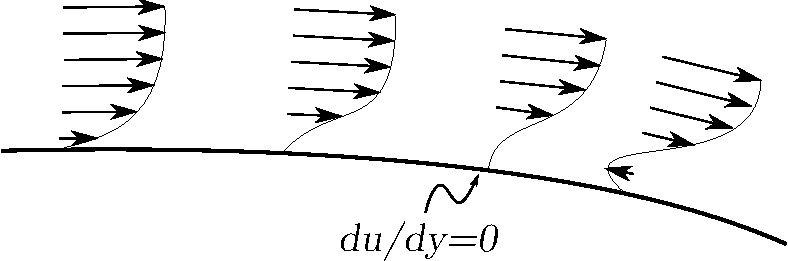
\includegraphics[width=0.8\textwidth]{clase12/separacion.pdf}
\caption{Mecanismo de separación de la capa límite.}
\label{fig:separacion}
\end{figure}

La Figura \ref{fig:separacion} muestra el mecanismo de separación de la capa límite.
El gradiente adverso de presión desacelera al flujo cerca de la pared, y lejos de la pared la inercia de $U_\infty$ arrastra la capa límite.
Por este efecto, la gradiente de velocidad sobre la placa disminuye, a tal punto que llega a ser cero ($\partial u/\partial y=0$).
Es en este punto donde se considera que el flujo se separa, ya que después de él hay un flujo en dirección contraria, que despega la capa límite.

\mbox{?`}Se acuerdan que el perfil de velocidad de una capa límite turbulenta tenía una gradiente de velocidad mayor que el perfil de Blasius cerca de la pared?
Si la gradiente es mayor, el mecanismo descrito por la Figura \ref{fig:separacion} demora más en separar el flujo (debe ``empujar'' el perfil desde una gradiente mayor).
Esta es la razón por la cual el flujo turbulento se demora más en separar.
De hecho, en las alas de aviones es muy común encontrar placas en la superficie que hacen las veces de generadores de turbulencia.
Al generar turbulencia, se retarda la separación, lo que es deseable para evitar el temido ``stall''.
